\documentclass[pra,aps,showpacs,groupedaddress,superscriptaddress,twocolumn,toc=flat]{revtex4-1}

\usepackage[colorlinks=true,linkcolor=blue,urlcolor=blue,citecolor=blue]{hyperref}

\usepackage[utf8x]{inputenc}
\usepackage{color}
\usepackage{bbm} 

\usepackage{amsfonts,amsmath,amssymb,stmaryrd}

\usepackage{graphicx}
\usepackage{subfigure}  % use for side-by-side figures
\usepackage{bbm} 
\usepackage{hyperref}
\usepackage{epsfig}
\usepackage{mathrsfs}
\usepackage{verbatim}
\usepackage{centernot}
\usepackage{ulem}
\usepackage{longtable}
\usepackage{nicefrac}
\usepackage[framemethod=tikz]{mdframed}

\begin{document}

\title{Tutorial on the Heisenberg model}

\begin{abstract}
In this tutorial we compare the differences between the spin $S=1/2$ and $S=1$ Heisenberg models on a chain lattice.


\end{abstract}

\maketitle

\section{Compiling the code}
We assume that the reader has already been able to successfully compile the code before, and is familiar with the Monte Carlo examples and tutorials provided by ALPSCore.
In the \texttt{cmake} variables  we make sure that the lattice variable is set to \texttt{chain}, the variable \texttt{CWINDOW} is switched \texttt{OFF}, and \texttt{UNIFORM} must be on. 
On \texttt{Linux} operating systems we can achieve this by going to the \texttt{build} directory, typing \texttt{ccmake .} and edit the corresponding variables. We are now in a position to recompile the code.
The simplest way to go through the tutorial is to copy and edit the parameter files provided in the \texttt{parameterfiles} directory. We set  \texttt{Lx = 32}, and work with periodic boundary conditions, \texttt{pbcx =1}.
We look at the Heisenberg model and set \texttt{Jzz=Jpm=1} (note the convention of the spin Hamiltonian with a factor $1/2$ explicitly preceding \texttt{Jpm}). There is no magnetic field, and we can set the inverse temperature to be equal to half of the system size.

\section{Spin-$1/2$ system}
We can choose a spin-$1/2$ system by setting $\texttt{nmax=1}$. The model should be \texttt{model="XXZ"}. Since the spin-$1/2$ Heisenberg chain is in a critical phase, we can set \texttt{Nmeasure=1}, and also \texttt{Nmeasure2=1} should be chosen because we want the level of statistics on the $S^z_0S^z_r$ and $(S^+_0S^-_r + \rm{h.c.})$ correlation functions to be comparable. For our purposes it should suffice to take 2 million sweeps, and $20\%$ thermalization sweeps. The correlation functions are expected to decay like a power-law (see below) and in an equal fashion owing to the Heisenberg symmetry. The spin stiffness is finite (and large), which can also be seen in the output of the code.

\section{Spin-$1$ system}
We can use the same parameters as before, but only need to change $\texttt{nmax=2}$. This has however a dramatic effect on the physics: the spin-1 Heisenberg chain is gapped, {\it i.e.}, there is a finite energy gap towards excitations and the correlation functions decay exponentially with distance. Note that there is in fact a hidden string order (Haldane), but we will not analyze this further. Indications of the gap are also seen in the vanishing spin stiffness.

The $S^z_0S^z_r$ and $(S^+_0S^-_r + \rm{h.c.)}$ correlation functions are shown in Fig.~\ref{fig:half} for a $S=1/2$ chain and in Fig.~\ref{fig:one} for a $S=1$ chain. In either case we showed the reflection of the Heisenberg symmetry in the correlation functions manifestly. The difference between the power-law behavior for the critical phase and the exponential behavior in the massive phase is apparent.
Note that for either model there is a "particle-hole" symmetry enforcing a total $\langle S^z\rangle=0$. 




\begin{figure}[h!]
\centering
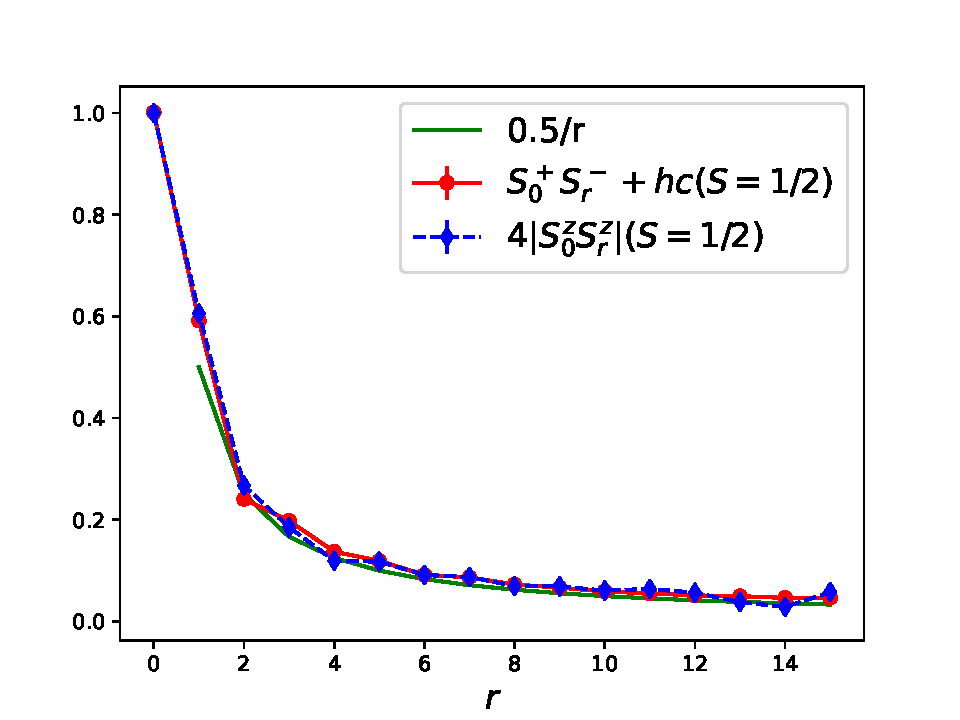
\includegraphics[width=0.6\linewidth]{fig_corr_half.pdf}
\caption{The $(S^+_0S^-_r + {\rm h.c.})$ and $S^z_0S^z_r$ correlation function as a function of separation $r$ for a spin $S=1/2$ Heisenberg chain shown over half the system size. 
The $S^z_0S^z_r$ correlation function has been rescaled by a factor of 4 and we took its absolute value to show the Heisenberg symmetry manifestly. 
According to bosonization, the behavior of these correlation functions is $\sim 1/(r)$ (green line), up to logarithmic corrections (the latter are not included). The coefficients for the smallest values of $r$ are known analytically from the Bethe Ansatz, but differ only slightly from 0.5.
Deviations for $r$-values close to half the system size are seen because of the periodic boundary conditions. } 
\label{fig:half}
\end{figure}

\begin{figure}[h!]
\centering
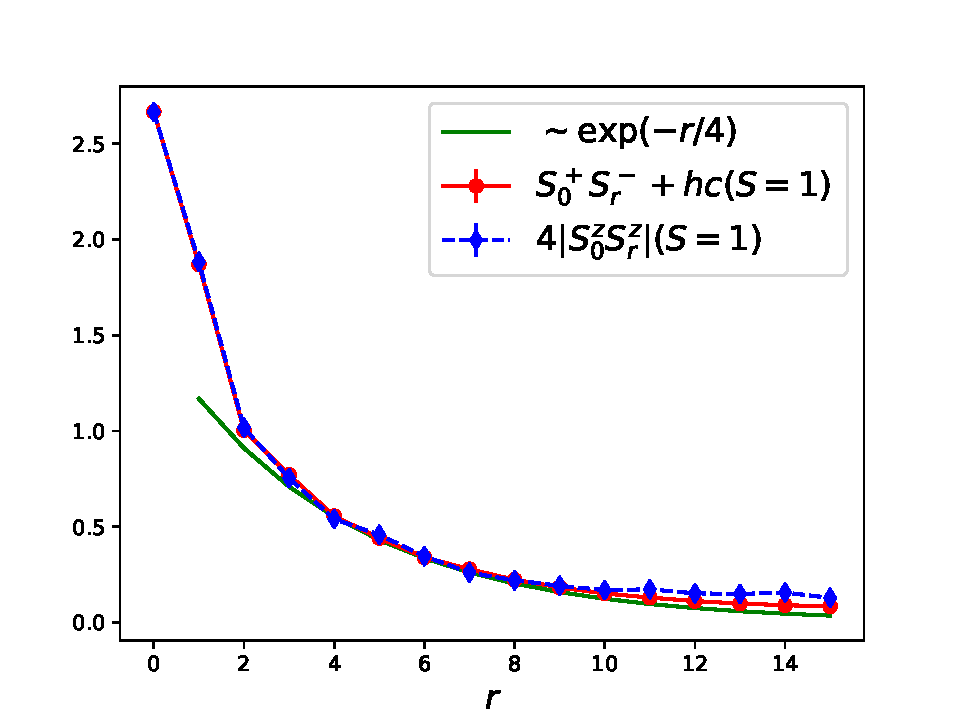
\includegraphics[width=0.6\linewidth]{fig_corr_one.pdf}
\caption{The $S^+_0S^-_r + {\rm h.c.}$ and $S^z_0S^z_r$ correlation function as a function of separation $r$ for a spin $S=1$ Heisenberg chain. The $S^z_0S^z_r$ correlation function has been rescaled by a factor of 4 and we took its absolute value to show the Heisenberg symmetry manifestly. The system is in a gapped phase, hence the shown correlation functions decay exponentially. At large distances the relative noise in the correlation functions can still be seen and longer runs are needed to reduce it.
} 
\label{fig:one}
\end{figure}


\end{document}
